\section{System Use-case Diagram}

\begin{figure}[H]
    \centering
    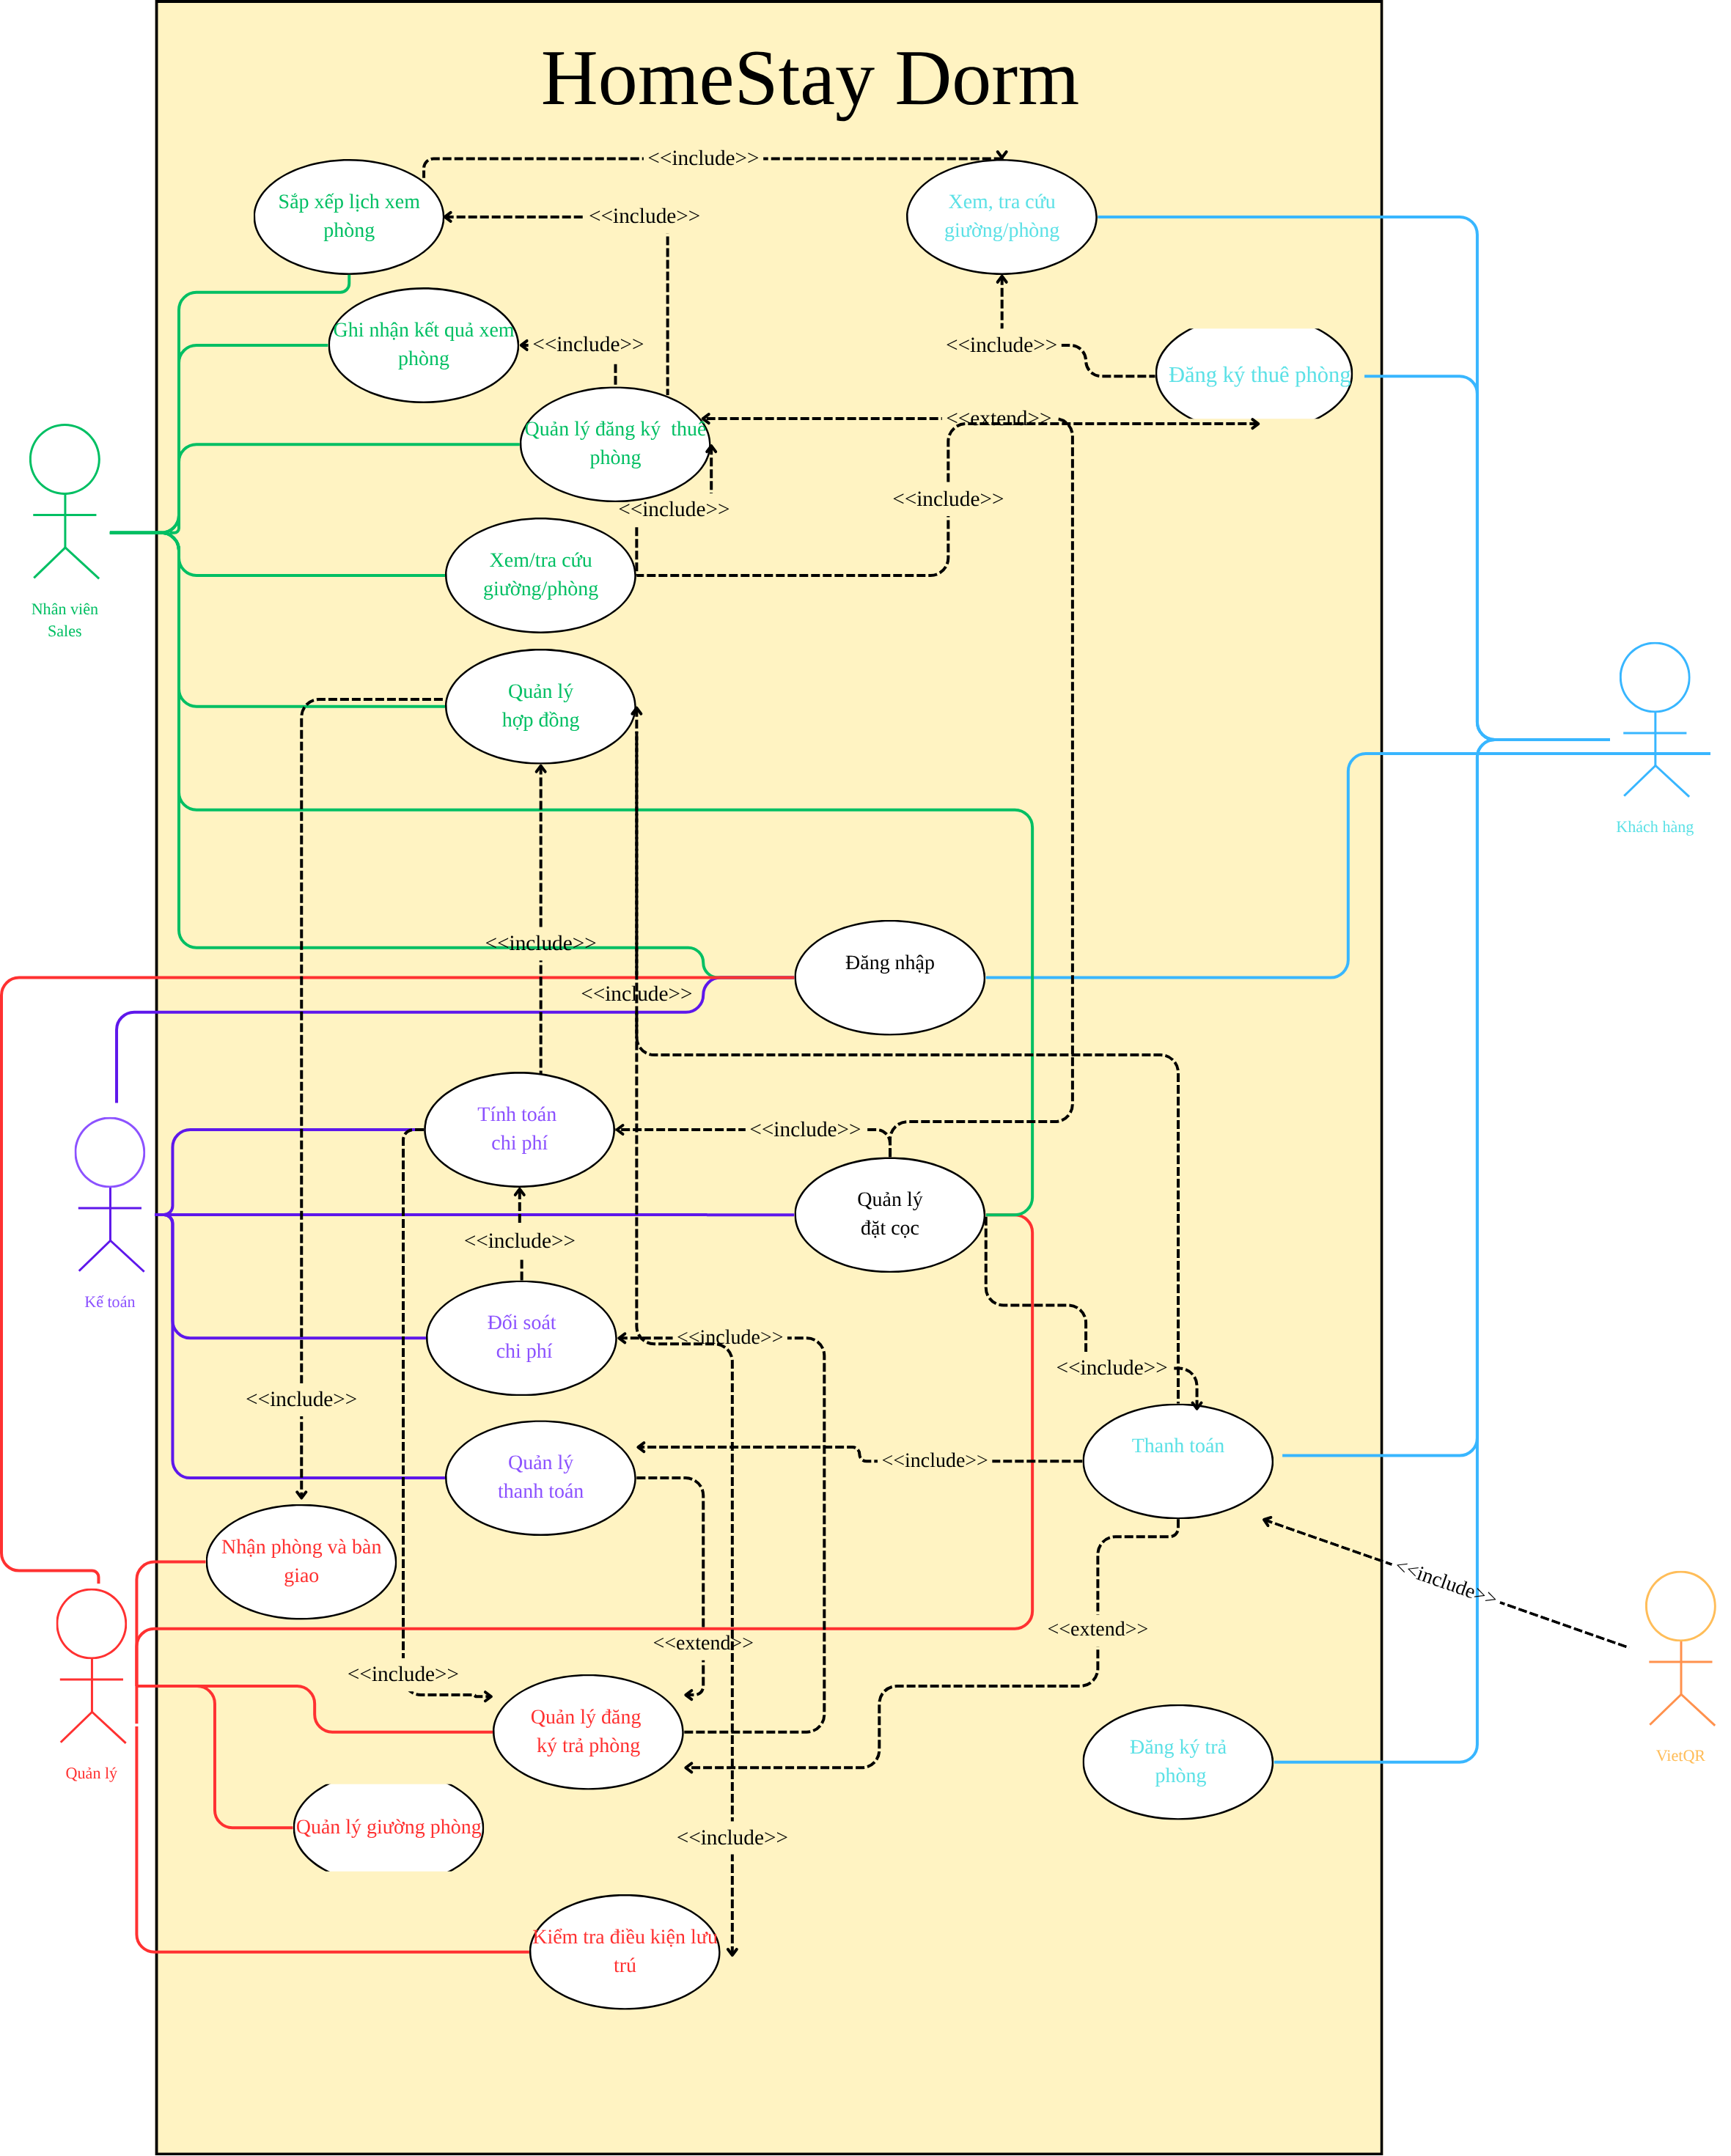
\includegraphics[width=0.98\textwidth]{images/SystemUseCase.png}
    \caption{Mô hình Use-case hệ thống}
\end{figure}
\newpage


\subsection{Đặc tả System Use Case}
% ============================================================
% SUC1
% ============================================================
\begin{table}[H]
\centering
\begin{tabularx}{\textwidth}{|>{\centering\arraybackslash\bfseries}m{3.5cm}|X|}
    \hline
    Use Case & {\centering\textbf{SUC1: Đăng nhập}\par} \\
    \hline
    Mô tả & Cho phép người dùng truy cập hệ thống để thực hiện các chức năng tương ứng với vai trò. \\
    \hline
    Actor &
    \vspace{0.3cm}
    \begin{itemize}
        \item Nhân viên Sales
        \item Kế toán
        \item Quản lý
        \item Khách hàng 
    \end{itemize} \\
    \hline
    Sự kiện kích hoạt & Người dùng chọn chức năng ``Đăng nhập''. \\
    \hline
    Tiền điều kiện & Người dùng đã có tài khoản. \\
    \hline
    Hậu điều kiện & Người dùng đăng nhập thành công vào hệ thống. \\
    \hline
    Dòng chính &
    \begin{enumerate}[leftmargin=*, nosep]
        \vspace{0.1cm}
        \item Hệ thống hiển thị màn hình đăng nhập.
        \item Người dùng nhập username và password.
        \item Hệ thống kiểm tra thông tin.
        \item Hệ thống xác thực thành công.
        \item Hệ thống chuyển vào màn hình chính.
        \item Kết thúc use case.
    \end{enumerate} \\
    \hline
    Dòng thay thế &
    \begin{itemize}[leftmargin=*, nosep, label=-]
        \vspace{0.1cm}
        \item \textbf{A1 -- Sai thông tin đăng nhập:} Hệ thống hiển thị lỗi; người dùng nhập lại.
        \item \textbf{A2 -- Quên mật khẩu:} Hệ thống hiển thị form nhập email; người dùng nhập email; hệ thống gửi link reset.
    \end{itemize} \\
    \hline
    Use-Case liên quan & Không. \\
    \hline
\end{tabularx}
\caption{Đặc tả SUC1: Đăng nhập}
\end{table}


\vspace{1cm}

% ============================================================
% SUC2
% ============================================================
\begin{table}[H]
\centering
\begin{tabularx}{\textwidth}{|>{\centering\arraybackslash\bfseries}m{3.5cm}|X|}
    \hline
    Use Case & {\centering\textbf{SUC2: Đăng ký thuê phòng}\par} \\
    \hline
    Mô tả & Khách hàng gửi yêu cầu thuê phòng tới hệ thống. \\
    \hline
    Actor &
    \begin{itemize}[leftmargin=*, nosep, label=\textbullet]
        \vspace{0.1cm}
        \item Khách hàng
    \end{itemize} \\
    \hline
    Sự kiện kích hoạt & Khách hàng chọn ``Đăng ký thuê phòng''. \\
    \hline
    Tiền điều kiện & Khách hàng đã đăng nhập. \\
    \hline
    Hậu điều kiện & Yêu cầu thuê được tạo. \\
    \hline
    Dòng chính &
    \begin{enumerate}[leftmargin=*, nosep]
        \vspace{0.1cm}
        \item Hệ thống hiển thị danh sách phòng.
        \item Khách hàng tra cứu phòng.
        \item Khách hàng chọn phòng.
        \item Khách hàng nhập thông tin thuê.
        \item Hệ thống lưu yêu cầu thuê.
        \item Kết thúc.
    \end{enumerate} \\
    \hline
    Dòng thay thế &
    \begin{itemize}[leftmargin=*, nosep, label=-]
        \vspace{0.1cm}
        \item \textbf{A1 -- Không có phòng phù hợp:} Hệ thống thông báo; kết thúc.
    \end{itemize} \\
    \hline
    Use-Case liên quan &
    \begin{itemize}[leftmargin=*, nosep, label=-]
        \vspace{0.1cm}
        \item \textit{(include)} Xem/tra cứu giường/phòng.
    \end{itemize} \\
    \hline
\end{tabularx}
\caption{Đặc tả SUC2: Đăng ký thuê phòng}
\end{table}


\vspace{1cm}

% ============================================================
% SUC3
% ============================================================
\begin{table}[H]
\centering
\begin{tabularx}{\textwidth}{|>{\centering\arraybackslash\bfseries}m{3.5cm}|X|}
    \hline
    Use Case & {\centering\textbf{SUC3: Quản lý đăng ký thuê phòng}\par} \\
    \hline
    Mô tả & Nhân viên Sales tiếp nhận yêu cầu thuê, tra cứu phòng phù hợp, sắp xếp lịch xem phòng và ghi nhận kết quả xem phòng của khách hàng. \\
    \hline
    Actor &
    \begin{itemize}[leftmargin=*, nosep, label=\textbullet]
        \vspace{0.1cm}
        \item Nhân viên Sales
    \end{itemize} \\
    \hline
    Sự kiện kích hoạt & Có yêu cầu thuê phòng từ khách hàng. \\
    \hline
    Tiền điều kiện & Nhân viên đã đăng nhập và có yêu cầu thuê. \\
    \hline
    Hậu điều kiện & Yêu cầu thuê được cập nhật trạng thái sau xem phòng; nếu khách đồng ý thuê thì sẵn sàng chuyển sang xử lý đặt cọc. \\
    \hline
    Dòng chính &
    \begin{enumerate}[leftmargin=*, nosep]
        \vspace{0.1cm}
        \item Hệ thống hiển thị danh sách yêu cầu thuê.
        \item Nhân viên chọn yêu cầu.
        \item Thực hiện \textbf{SUC13} để tra cứu phòng/giường phù hợp.
        \item Thực hiện \textbf{SUC14} để sắp xếp lịch xem phòng với khách hàng.
        \item Đến lịch hẹn, thực hiện \textbf{SUC15} để ghi nhận kết quả xem phòng.
        \item Nếu khách hàng đồng ý thuê, nhân viên xác nhận nhu cầu thuê trên hệ thống.
        \item Hệ thống cập nhật trạng thái yêu cầu và tạo cơ sở để thực hiện \textbf{SUC4}.
        \item Kết thúc.
    \end{enumerate} \\
    \hline
    Dòng thay thế &
    \begin{itemize}[leftmargin=*, nosep, label=-]
        \vspace{0.1cm}
        \item \textbf{A1 -- Không còn phòng phù hợp:} Hệ thống thông báo; nhân viên tư vấn lại phòng/giường khác hoặc kết thúc yêu cầu.
        \item \textbf{A2 -- Khách không tham gia hoặc không đồng ý sau khi xem phòng:} Nhân viên ghi nhận kết quả; hệ thống cập nhật trạng thái yêu cầu là chưa tiếp tục thuê.
    \end{itemize} \\
    \hline
    Use-Case liên quan &
    \begin{itemize}[leftmargin=*, nosep, label=-]
        \vspace{0.1cm}
        \item \textit{(include)} Xem/tra cứu giường/phòng.
        \item \textit{(include)} Sắp xếp lịch xem phòng.
        \item \textit{(include)} Ghi nhận kết quả xem phòng.
        \item \textit{(extend)} Quản lý đặt cọc.
\end{itemize} \\
    \hline
\end{tabularx}
\caption{Đặc tả SUC3: Quản lý đăng ký thuê phòng}
\end{table}



\vspace{1cm}

% ============================================================
% SUC4
% ============================================================
\begin{table}[H]
\centering
\begin{tabularx}{\textwidth}{|>{\centering\arraybackslash\bfseries}m{3.5cm}|X|}
    \hline
    Use Case & {\centering\textbf{SUC4: Quản lý đặt cọc}\par} \\
    \hline
    Mô tả & Thực hiện tạo và xử lý yêu cầu đặt cọc cho việc thuê phòng. \\
    \hline
    Actor &
    \begin{itemize}[leftmargin=*, nosep, label=\textbullet]
        \vspace{0.1cm}
        \item Nhân viên Sales
        \item Kế toán
        \item Quản lý
    \end{itemize} \\
    \hline
    Sự kiện kích hoạt & Yêu cầu thuê phòng được chấp nhận. \\
    \hline
    Tiền điều kiện & Yêu cầu thuê đã được xác nhận và người dùng đã đăng nhập hợp lệ. \\
    \hline
    Hậu điều kiện & Đặt cọc được ghi nhận thành công. \\
    \hline
    Dòng chính &
    \begin{enumerate}[leftmargin=*, nosep]
        \vspace{0.1cm}
        \item Nhân viên tạo yêu cầu đặt cọc.
        \item Hệ thống hiển thị thông tin đặt cọc.
        \item Kế toán kiểm tra và nhập số tiền cọc.
        \item Hệ thống xác nhận số tiền.
        \item Thực hiện thanh toán.
        \item Hệ thống lưu trạng thái đặt cọc.
        \item Kết thúc.
    \end{enumerate} \\
    \hline
    Dòng thay thế &
    \begin{itemize}[leftmargin=*, nosep, label=-]
        \vspace{0.1cm}
        \item \textbf{A1 -- Thanh toán thất bại:} Hệ thống thông báo lỗi; cho phép thực hiện lại.
    \end{itemize} \\
    \hline
    Use-Case liên quan &
    \begin{itemize}[leftmargin=*, nosep, label=-]
        \vspace{0.1cm}
        \item \textit{(include)} Thanh toán.
        \item \textit{(include)} Tính toán chi phí.
\end{itemize} \\
    \hline
\end{tabularx}
\caption{Đặc tả SUC4: Quản lý đặt cọc}
\end{table}


\vspace{1cm}

% ============================================================
% SUC5
% ============================================================
\begin{table}[H]
\centering
\begin{tabularx}{\textwidth}{|>{\centering\arraybackslash\bfseries}m{3.5cm}|X|}
    \hline
    Use Case & {\centering\textbf{SUC5: Thanh toán}\par} \\
    \hline
    Mô tả & Thực hiện giao dịch thanh toán cho các nghiệp vụ trong hệ thống. \\
    \hline
    Actor &
    \begin{itemize}[leftmargin=*, nosep, label=\textbullet]
        \vspace{0.1cm}
        \item Khách hàng
        \item VietQR
    \end{itemize} \\
    \hline
    Sự kiện kích hoạt & Có yêu cầu thanh toán từ hệ thống. \\
    \hline
    Tiền điều kiện & Có giao dịch cần thanh toán. \\
    \hline
    Hậu điều kiện & Giao dịch thanh toán thành công hoặc thất bại được ghi nhận. \\
    \hline
    Dòng chính &
    \begin{enumerate}[leftmargin=*, nosep]
        \vspace{0.1cm}
        \item Hệ thống hiển thị thông tin thanh toán.
        \item Khách hàng chọn phương thức thanh toán.
        \item Hệ thống gửi yêu cầu tới VietQR.
        \item VietQR xử lý giao dịch.
        \item Hệ thống nhận kết quả.
        \item Hệ thống cập nhật trạng thái thanh toán.
        \item Kết thúc.
    \end{enumerate} \\
    \hline
    Dòng thay thế &
    \begin{itemize}[leftmargin=*, nosep, label=-]
        \vspace{0.1cm}
        \item \textbf{A1 -- Thanh toán thất bại:} Hệ thống hiển thị lỗi; cho phép thanh toán lại.
        \item \textbf{A2 -- Timeout / lỗi kết nối VietQR:} Hệ thống thông báo lỗi; giao dịch bị hủy.
    \end{itemize} \\
    \hline
    Use-Case liên quan &
    \begin{itemize}[leftmargin=*, nosep, label=-]
        \vspace{0.1cm}
        \item \textit{(include)} Quản lý thanh toán.
\end{itemize} \\
    \hline
\end{tabularx}
\caption{Đặc tả SUC5: Thanh toán}
\end{table}



\vspace{1cm}

% ============================================================
% SUC6
% ============================================================
\begin{table}[H]
\centering
\begin{tabularx}{\textwidth}{|>{\centering\arraybackslash\bfseries}m{3.5cm}|X|}
    \hline
    Use Case & {\centering\textbf{SUC6: Quản lý thanh toán}\par} \\
    \hline
    Mô tả & Quản lý và xử lý các giao dịch thanh toán trong hệ thống. \\
    \hline
    Actor &
    \begin{itemize}[leftmargin=*, nosep, label=\textbullet]
        \vspace{0.1cm}
        \item Kế toán
    \end{itemize} \\
    \hline
    Sự kiện kích hoạt & Có giao dịch thanh toán phát sinh. \\
    \hline
    Tiền điều kiện & Có dữ liệu giao dịch. \\
    \hline
    Hậu điều kiện & Giao dịch được ghi nhận và xử lý. \\
    \hline
    Dòng chính &
    \begin{enumerate}[leftmargin=*, nosep]
        \vspace{0.1cm}
        \item Hệ thống nhận thông tin giao dịch.
        \item Kế toán kiểm tra giao dịch.
        \item Hệ thống đối chiếu thông tin.
        \item Kế toán xác nhận giao dịch.
        \item Hệ thống lưu vào hệ thống.
        \item Kết thúc.
    \end{enumerate} \\
    \hline
    Dòng thay thế &
    \begin{itemize}[leftmargin=*, nosep, label=-]
        \vspace{0.1cm}
        \item \textbf{A1 -- Sai lệch giao dịch:} Hệ thống thông báo lỗi; kế toán kiểm tra lại.
        \item \textbf{A2 -- Giao dịch bị hủy:} Hệ thống cập nhật trạng thái hủy.
    \end{itemize} \\
    \hline
    Use-Case liên quan &
    \begin{itemize}[leftmargin=*, nosep, label=-]
        \vspace{0.1cm}
        \item \textit{(được include bởi)} Thanh toán.
\end{itemize} \\
    \hline
\end{tabularx}
\caption{Đặc tả SUC6: Quản lý thanh toán}
\end{table}

\vspace{1cm}

% ============================================================
% SUC7
% ============================================================
\begin{table}[H]
\centering
\begin{tabularx}{\textwidth}{|>{\centering\arraybackslash\bfseries}m{3.5cm}|X|}
    \hline
    Use Case & {\centering\textbf{SUC7: Quản lý hợp đồng}\par} \\
    \hline
    Mô tả & Lập, xác nhận và lưu hợp đồng thuê phòng sau khi khách hàng đã đặt cọc và đủ điều kiện lưu trú; đồng thời chuyển thông tin cho bước nhận phòng/bàn giao. \\
    \hline
    Actor &
    \begin{itemize}[leftmargin=*, nosep, label=\textbullet]
        \vspace{0.1cm}
        \item Nhân viên Sales
    \end{itemize} \\
    \hline
    Sự kiện kích hoạt & Khách hàng hoàn tất đặt cọc và đủ điều kiện thuê. \\
    \hline
    Tiền điều kiện & Khách hàng đã đặt cọc, đã được kiểm tra điều kiện lưu trú và nhân viên Sales đã đăng nhập. \\
    \hline
    Hậu điều kiện & Hợp đồng được tạo, lưu trong hệ thống và sẵn sàng cho bước nhận phòng/bàn giao. \\
    \hline
    Dòng chính &
    \begin{enumerate}[leftmargin=*, nosep]
        \vspace{0.1cm}
        \item Nhân viên chọn tạo hợp đồng.
        \item Hệ thống hiển thị thông tin khách hàng, phòng/giường, trạng thái đặt cọc và hồ sơ lưu trú.
        \item Thực hiện \textbf{SUC16} để kiểm tra điều kiện lưu trú trước khi lập hợp đồng.
        \item Thực hiện \textbf{SUC9} để tính các khoản chi phí cần thu khi ký hợp đồng.
        \item Nhân viên nhập các thông tin hợp đồng.
        \item Thực hiện \textbf{SUC5} nếu cần thu thêm tiền khi ký hợp đồng.
        \item Hệ thống sinh mã hợp đồng và lưu hợp đồng.
        \item Hệ thống chuyển thông tin cho quản lý để thực hiện \textbf{SUC17}.
        \item Kết thúc.
    \end{enumerate} \\
    \hline
    Dòng thay thế &
    \begin{itemize}[leftmargin=*, nosep, label=-]
        \vspace{0.1cm}
        \item \textbf{A1 -- Thông tin hợp đồng không hợp lệ:} Hệ thống thông báo lỗi; nhân viên nhập lại.
        \item \textbf{A2 -- Khách hàng không đủ điều kiện lưu trú:} Hệ thống không cho phép lập hợp đồng; ghi nhận kết quả kiểm tra và kết thúc.
        \item \textbf{A3 -- Thanh toán khi ký hợp đồng không thành công:} Hệ thống thông báo lỗi; hợp đồng chưa được kích hoạt.
    \end{itemize} \\
    \hline
    Use-Case liên quan &
    \begin{itemize}[leftmargin=*, nosep, label=-]
        \vspace{0.1cm}
        \item \textit{(include)} Kiểm tra điều kiện lưu trú.
        \item \textit{(include)} Tính toán chi phí.
        \item \textit{(include)} Thanh toán.
        \item \textit{(include)} Nhận phòng và bàn giao.
\end{itemize} \\
    \hline
\end{tabularx}
\caption{Đặc tả SUC7: Quản lý hợp đồng}
\end{table}



\vspace{1cm}

% ============================================================
% SUC8
% ============================================================
\begin{table}[H]
\centering
\begin{tabularx}{\textwidth}{|>{\centering\arraybackslash\bfseries}m{3.5cm}|X|}
    \hline
    Use Case & {\centering\textbf{SUC8: Đối soát chi phí}\par} \\
    \hline
    Mô tả & Thực hiện đối soát chi phí khi khách trả phòng, tổng hợp số tiền khách phải thanh toán thêm hoặc được hoàn lại dựa trên kết quả tính toán chi phí. \\
    \hline
    Actor &
    \begin{itemize}[leftmargin=*, nosep, label=\textbullet]
        \vspace{0.1cm}
        \item Kế toán
    \end{itemize} \\
    \hline
    Sự kiện kích hoạt & Có yêu cầu trả phòng. \\
    \hline
    Tiền điều kiện & Có dữ liệu thuê phòng và người dùng đã đăng nhập. \\
    \hline
    Hậu điều kiện & Kết quả đối soát chi phí được xác định và lưu để phục vụ quyết toán trả phòng. \\
    \hline
    Dòng chính &
    \begin{enumerate}[leftmargin=*, nosep]
        \vspace{0.1cm}
        \item Hệ thống hiển thị thông tin thuê.
        \item Kế toán kiểm tra thời gian thuê, tình trạng phòng và thông tin đặt cọc.
        \item Thực hiện \textbf{SUC9} để tính các khoản chi phí liên quan.
        \item Hệ thống tổng hợp các khoản phải thu thêm hoặc phải hoàn lại cho khách hàng.
        \item Kế toán xác nhận kết quả đối soát.
        \item Hệ thống lưu kết quả đối soát.
        \item Kết thúc.
    \end{enumerate} \\
    \hline
    Dòng thay thế &
    \begin{itemize}[leftmargin=*, nosep, label=-]
        \vspace{0.1cm}
        \item \textbf{A1 -- Thiếu dữ liệu:} Hệ thống thông báo lỗi; không thực hiện tiếp.
        \item \textbf{A2 -- Dữ liệu bàn giao chưa đầy đủ:} Hệ thống tạm dừng đối soát; yêu cầu cập nhật lại tình trạng phòng/tài sản.
    \end{itemize} \\
    \hline
    Use-Case liên quan &
    \begin{itemize}[leftmargin=*, nosep, label=-]
        \vspace{0.1cm}
        \item \textit{(include)} Tính toán chi phí.
        \item \textit{(include)} trong Quản lý đăng ký trả phòng.
\end{itemize} \\
    \hline
\end{tabularx}
\caption{Đặc tả SUC8: Đối soát chi phí}
\end{table}

\vspace{1cm}

% ============================================================
% SUC9
% ============================================================
\begin{table}[H]
\centering
\begin{tabularx}{\textwidth}{|>{\centering\arraybackslash\bfseries}m{3.5cm}|X|}
    \hline
    Use Case & {\centering\textbf{SUC9: Tính toán chi phí}\par} \\
    \hline
    Mô tả & Thực hiện tính toán các khoản chi phí liên quan đến thuê phòng, bao gồm tiền cọc, tiền thuê và các chi phí phát sinh. \\
    \hline
    Actor &
    \begin{itemize}[leftmargin=*, nosep, label=\textbullet]
        \vspace{0.1cm}
        \item Kế toán
    \end{itemize} \\
    \hline
    Sự kiện kích hoạt & Có yêu cầu xác định chi phí từ hệ thống (đặt cọc, lập hợp đồng hoặc trả phòng). \\
    \hline
    Tiền điều kiện & Có dữ liệu liên quan đến thuê phòng (giá phòng, thời gian thuê, thông tin khách hàng) và người dùng đã đăng nhập. \\
    \hline
    Hậu điều kiện & Các khoản chi phí được tính toán và cung cấp cho use case gọi. \\
    \hline
    Dòng chính &
    \begin{enumerate}[leftmargin=*, nosep]
        \vspace{0.1cm}
        \item Hệ thống nhận yêu cầu tính toán chi phí.
        \item Hệ thống xác định loại nghiệp vụ (đặt cọc / hợp đồng / trả phòng).
        \item Hệ thống truy xuất dữ liệu liên quan.
        \item Hệ thống tính toán chi phí theo nghiệp vụ:
        \begin{itemize}[leftmargin=*, nosep, label=\textbullet]
            \item Tiền cọc (nếu đặt cọc).
            \item Tiền thuê (nếu lập hợp đồng).
            \item Chi phí phát sinh (nếu trả phòng).
        \end{itemize}
        \item Hệ thống tổng hợp kết quả.
        \item Hệ thống trả kết quả cho use case gọi.
        \item Kết thúc.
    \end{enumerate} \\
    \hline
    Dòng thay thế &
    \begin{itemize}[leftmargin=*, nosep, label=-]
        \vspace{0.1cm}
        \item \textbf{A1 -- Thiếu dữ liệu:} Hệ thống phát hiện thiếu thông tin (giá phòng / thời gian thuê / hợp đồng); hệ thống thông báo lỗi; không thực hiện tính toán.
        \item \textbf{A2 -- Dữ liệu không hợp lệ:} Hệ thống phát hiện dữ liệu sai (thời gian âm, giá không hợp lệ); hệ thống yêu cầu kiểm tra lại; kết thúc.
        \item \textbf{A3 -- Không có chi phí phát sinh:} Hệ thống xác định không có khoản phụ phí; hệ thống trả kết quả chỉ gồm chi phí cơ bản.
    \end{itemize} \\
    \hline
    Use-Case liên quan &
    \begin{itemize}[leftmargin=*, nosep, label=-]
        \vspace{0.1cm}
        \item \textit{(được include bởi)} Quản lý đăng ký trả phòng.
        \item \textit{(được include bởi)} Quản lý đặt cọc.
        \item \textit{(được include bởi)} Quản lý hợp đồng.
\end{itemize} \\
    \hline
\end{tabularx}
\caption{Đặc tả SUC9: Tính toán chi phí}
\end{table}


\vspace{1cm}

% ============================================================
% SUC10
% ============================================================
\begin{table}[H]
\centering
\begin{tabularx}{\textwidth}{|>{\centering\arraybackslash\bfseries}m{3.5cm}|X|}
    \hline
    Use Case & {\centering\textbf{SUC10: Đăng ký trả phòng}\par} \\
    \hline
    Mô tả & Khách hàng gửi yêu cầu trả phòng tới hệ thống. \\
    \hline
    Actor &
    \begin{itemize}[leftmargin=*, nosep, label=\textbullet]
        \vspace{0.1cm}
        \item Khách hàng
    \end{itemize} \\
    \hline
    Sự kiện kích hoạt & Khách hàng chọn chức năng ``Đăng ký trả phòng''. \\
    \hline
    Tiền điều kiện & Khách hàng đang có hợp đồng thuê và đã đăng nhập. \\
    \hline
    Hậu điều kiện & Yêu cầu trả phòng được tạo. \\
    \hline
    Dòng chính &
    \begin{enumerate}[leftmargin=*, nosep]
        \vspace{0.1cm}
        \item Hệ thống hiển thị thông tin thuê.
        \item Khách hàng chọn trả phòng.
        \item Khách hàng xác nhận.
        \item Hệ thống tạo yêu cầu trả phòng.
        \item Kết thúc.
    \end{enumerate} \\
    \hline
    Dòng thay thế &
    \begin{itemize}[leftmargin=*, nosep, label=-]
        \vspace{0.1cm}
        \item \textbf{A1 -- Không có hợp đồng thuê:} Hệ thống thông báo; kết thúc.
    \end{itemize} \\
    \hline
    Use-Case liên quan & Không. \\
    \hline
\end{tabularx}
\caption{Đặc tả SUC10: Đăng ký trả phòng}
\end{table}



\vspace{1cm}

% ============================================================
% SUC11
% ============================================================
\begin{table}[H]
\centering
\begin{tabularx}{\textwidth}{|>{\centering\arraybackslash\bfseries}m{3.5cm}|X|}
    \hline
    Use Case & {\centering\textbf{SUC11: Quản lý đăng ký trả phòng}\par} \\
    \hline
    Mô tả & Tiếp nhận và xử lý yêu cầu trả phòng của khách hàng, bao gồm đối soát chi phí, quyết toán thanh toán/hoàn cọc, thanh lý hợp đồng và cập nhật kết thúc lưu trú. \\
    \hline
    Actor &
    \begin{itemize}[leftmargin=*, nosep, label=\textbullet]
        \vspace{0.1cm}
        \item Quản lý
    \end{itemize} \\
    \hline
    Sự kiện kích hoạt & Có yêu cầu trả phòng từ khách hàng. \\
    \hline
    Tiền điều kiện &
    \begin{itemize}[leftmargin=*, nosep, label=\textbullet]
        \vspace{0.1cm}
        \item Có yêu cầu trả phòng.
        \item Quản lý đã đăng nhập.
    \end{itemize} \\
    \hline
    Hậu điều kiện & Trả phòng được xử lý hoàn tất; hợp đồng được thanh lý và trạng thái phòng/giường được cập nhật. \\
    \hline
    Dòng chính &
    \begin{enumerate}[leftmargin=*, nosep]
        \vspace{0.1cm}
        \item Hệ thống hiển thị danh sách yêu cầu trả phòng.
        \item Quản lý chọn yêu cầu.
        \item Hệ thống hiển thị thông tin thuê, hợp đồng, tiền cọc và tình trạng phòng hiện tại.
        \item Thực hiện \textbf{SUC8} để đối soát chi phí trả phòng.
        \item Hệ thống hiển thị kết quả đối soát, bao gồm số tiền cần thu thêm hoặc số tiền cần hoàn lại.
        \item Nếu có phát sinh thanh toán/hoàn tiền, thực hiện \textbf{SUC5}.
        \item Quản lý ký xác nhận biên bản trả phòng và thanh lý hợp đồng với khách hàng.
        \item Quản lý ghi nhận việc thu hồi chìa khóa/thẻ ra vào và cập nhật bàn giao tài sản.
        \item Hệ thống cập nhật trạng thái hợp đồng là đã thanh lý và trạng thái phòng/giường là trống.
        \item Hệ thống thông báo hoàn tất trả phòng.
        \item Kết thúc.
    \end{enumerate} \\
    \hline
    Dòng thay thế &
    \begin{itemize}[leftmargin=*, nosep, label=-]
        \vspace{0.1cm}
        \item \textbf{A1 -- Thanh toán/hoàn tiền chưa hoàn tất:} Hệ thống giữ trạng thái xử lý trả phòng; chưa cho phép thanh lý hợp đồng.
        \item \textbf{A2 -- Khách chưa bàn giao đủ chìa khóa, thẻ ra vào hoặc tài sản:} Quản lý ghi nhận thiếu sót; yêu cầu khách hoàn tất bàn giao trước khi tiếp tục.
        \item \textbf{A3 -- Lỗi cập nhật trạng thái hợp đồng hoặc phòng:} Hệ thống thông báo lỗi; trả phòng chưa được hoàn tất.
    \end{itemize} \\
    \hline
    Use-Case liên quan &
    \begin{itemize}[leftmargin=*, nosep, label=-]
        \vspace{0.1cm}
        \item \textit{(include)} Đối soát chi phí.
        \item \textit{(extend)} Thanh toán.
\end{itemize} \\
    \hline
\end{tabularx}
\caption{Đặc tả SUC11: Quản lý đăng ký trả phòng}
\end{table}


\vspace{1cm}

% ============================================================
% SUC12
% ============================================================
\begin{table}[H]
\centering
\begin{tabularx}{\textwidth}{|>{\centering\arraybackslash\bfseries}m{3.5cm}|X|}
    \hline
    Use Case & {\centering\textbf{SUC12: Quản lý giường phòng}\par} \\
    \hline
    Mô tả & Quản lý thông tin giường/phòng (thêm, sửa, xóa, xem). \\
    \hline
    Actor &
    \begin{itemize}[leftmargin=*, nosep, label=\textbullet]
        \vspace{0.1cm}
        \item Quản lý
    \end{itemize} \\
    \hline
    Sự kiện kích hoạt & Quản lý chọn chức năng quản lý giường/phòng. \\
    \hline
    Tiền điều kiện & Quản lý đã đăng nhập. \\
    \hline
    Hậu điều kiện & Thông tin giường/phòng được cập nhật. \\
    \hline
    Dòng chính &
    \begin{enumerate}[leftmargin=*, nosep]
        \vspace{0.1cm}
        \item Hệ thống hiển thị danh sách giường/phòng.
        \item Quản lý chọn thao tác: thêm / sửa / xóa / xem.
        \item Quản lý chọn thông tin để xem / nhập thông tin mới / chỉnh sửa thông tin đã có / xóa thông tin cũ.
        \item Hệ thống mở dữ liệu xem / lưu dữ liệu mới / cập nhật dữ liệu tương ứng / xóa dữ liệu.
        \item Kết thúc.
    \end{enumerate} \\
    \hline
    Dòng thay thế &
    \begin{itemize}[leftmargin=*, nosep, label=-]
        \vspace{0.1cm}
        \item \textbf{A1 -- Dữ liệu không hợp lệ:} Hệ thống thông báo lỗi; nhập lại.
        \item \textbf{A2 -- Không thể xóa (đang được sử dụng):} Hệ thống từ chối; kết thúc.
    \end{itemize} \\
    \hline
    Use-Case liên quan & Không. \\
    \hline
\end{tabularx}
\caption{Đặc tả SUC12: Quản lý giường phòng}
\end{table}


\vspace{1cm}

% ============================================================
% SUC13
% ============================================================
\begin{table}[H]
\centering
\begin{tabularx}{\textwidth}{|>{\centering\arraybackslash\bfseries}m{3.5cm}|X|}
    \hline
    Use Case & {\centering\textbf{SUC13: Xem/tra cứu giường/phòng}\par} \\
    \hline
    Mô tả & Cho phép người dùng tra cứu thông tin phòng/giường. \\
    \hline
    Actor &
    \begin{itemize}[leftmargin=*, nosep, label=\textbullet]
        \vspace{0.1cm}
        \item Nhân viên Sales
        \item Khách hàng
    \end{itemize} \\
    \hline
    Sự kiện kích hoạt & Người dùng chọn chức năng tra cứu. \\
    \hline
    Tiền điều kiện & Người dùng đã đăng nhập (có thể bỏ nếu hệ thống cho phép public). \\
    \hline
    Hậu điều kiện & Danh sách phòng được hiển thị. \\
    \hline
    Dòng chính &
    \begin{enumerate}[leftmargin=*, nosep]
        \vspace{0.1cm}
        \item Hệ thống hiển thị danh sách phòng.
        \item Người dùng nhập tiêu chí tìm kiếm.
        \item Hệ thống lọc dữ liệu.
        \item Hệ thống hiển thị kết quả.
        \item Người dùng xem chi tiết phòng.
        \item Kết thúc.
    \end{enumerate} \\
    \hline
    Dòng thay thế &
    \begin{itemize}[leftmargin=*, nosep, label=-]
        \vspace{0.1cm}
        \item \textbf{A1 -- Không có kết quả:} Hệ thống thông báo; cho phép tìm lại.
    \end{itemize} \\
    \hline
    Use-Case liên quan &
    \begin{itemize}[leftmargin=*, nosep, label=-]
        \vspace{0.1cm}
        \item \textit{(được include bởi)} Quản lý đăng ký thuê phòng.
        \item \textit{(được include bởi)} Đăng ký thuê phòng.
        \item \textit{(được include bởi)} Sắp xếp lịch xem phòng.
\end{itemize} \\
    \hline
\end{tabularx}
\caption{Đặc tả SUC13: Xem/tra cứu giường/phòng}
\end{table}

\vspace{1cm}

% ============================================================
% SUC14
% ============================================================
\begin{table}[H]
\centering
\begin{tabularx}{\textwidth}{|>{\centering\arraybackslash\bfseries}m{3.5cm}|X|}
    \hline
    Use Case & {\centering\textbf{SUC14: Sắp xếp lịch xem phòng}\par} \\
    \hline
    Mô tả & Nhân viên Sales sắp xếp lịch xem phòng với khách hàng và lưu lịch hẹn trên hệ thống. \\
    \hline
    Actor &
    \begin{itemize}[leftmargin=*, nosep, label=\textbullet]
        \vspace{0.1cm}
        \item Nhân viên Sales
    \end{itemize} \\
    \hline
    Sự kiện kích hoạt & Có yêu cầu thuê cần hẹn lịch xem phòng. \\
    \hline
    Tiền điều kiện & Yêu cầu thuê đang ở trạng thái xử lý và đã có phòng/giường phù hợp. \\
    \hline
    Hậu điều kiện & Lịch xem phòng được tạo và thông tin lịch hẹn được lưu trên hệ thống. \\
    \hline
    Dòng chính &
    \begin{enumerate}[leftmargin=*, nosep]
        \vspace{0.1cm}
        \item Nhân viên mở yêu cầu thuê cần sắp lịch xem phòng.
        \item Hệ thống hiển thị thông tin khách hàng, phòng/giường và các khung giờ khả dụng.
        \item Nhân viên trao đổi với khách hàng và chọn thời gian xem phòng phù hợp.
        \item Hệ thống ghi nhận lịch xem phòng.
        \item Hệ thống gửi hoặc hiển thị thông tin lịch hẹn cho khách hàng.
        \item Kết thúc.
    \end{enumerate} \\
    \hline
    Dòng thay thế &
    \begin{itemize}[leftmargin=*, nosep, label=-]
        \vspace{0.1cm}
        \item \textbf{A1 -- Không còn khung giờ phù hợp:} Hệ thống thông báo; nhân viên chọn thời gian khác hoặc tạm hoãn lịch.
        \item \textbf{A2 -- Khách hàng hủy lịch hẹn:} Hệ thống cập nhật trạng thái lịch là đã hủy; kết thúc.
    \end{itemize} \\
    \hline
    Use-Case liên quan &
    \begin{itemize}[leftmargin=*, nosep, label=-]
        \vspace{0.1cm}
        \item \textit{(include)} Xem/tra cứu giường/phòng.
        \item \textit{(được include bởi)} Quản lý đăng ký thuê phòng.
\end{itemize} \\
    \hline
\end{tabularx}
\caption{Đặc tả SUC14: Sắp xếp lịch xem phòng}
\end{table}



% ===================   =========================================
% SUC15
% ============================================================
\begin{table}[H]
\centering
\begin{tabularx}{\textwidth}{|>{\centering\arraybackslash\bfseries}m{3.5cm}|X|}
    \hline
    Use Case & {\centering\textbf{SUC15: Ghi nhận kết quả xem phòng}\par} \\
    \hline
    Mô tả & Nhân viên Sales ghi nhận kết quả buổi xem phòng và nhu cầu thuê của khách hàng sau khi xem thực tế. \\
    \hline
    Actor &
    \begin{itemize}[leftmargin=*, nosep, label=\textbullet]
        \vspace{0.1cm}
        \item Nhân viên Sales
    \end{itemize} \\
    \hline
    Sự kiện kích hoạt & Đến lịch xem phòng đã được tạo trước đó. \\
    \hline
    Tiền điều kiện & Đã có lịch xem phòng hợp lệ. \\
    \hline
    Hậu điều kiện & Kết quả xem phòng và nhu cầu tiếp tục thuê của khách hàng được lưu trên hệ thống. \\
    \hline
    Dòng chính &
    \begin{enumerate}[leftmargin=*, nosep]
        \vspace{0.1cm}
        \item Nhân viên mở lịch xem phòng cần xử lý.
        \item Hệ thống hiển thị thông tin lịch hẹn và phòng/giường đã xem.
        \item Nhân viên ghi nhận tình trạng buổi xem phòng và phản hồi của khách hàng.
        \item Nhân viên chọn kết quả: khách đồng ý thuê, cần tư vấn thêm hoặc không tiếp tục thuê.
        \item Hệ thống lưu kết quả và cập nhật trạng thái yêu cầu thuê.
        \item Kết thúc.
    \end{enumerate} \\
    \hline
    Dòng thay thế &
    \begin{itemize}[leftmargin=*, nosep, label=-]
        \vspace{0.1cm}
        \item \textbf{A1 -- Khách không đến xem phòng:} Hệ thống ghi nhận vắng mặt; nhân viên chọn sắp lịch lại hoặc kết thúc yêu cầu.
        \item \textbf{A2 -- Khách không đồng ý thuê:} Hệ thống lưu kết quả; yêu cầu thuê chuyển sang trạng thái không tiếp tục.
    \end{itemize} \\
    \hline
    Use-Case liên quan &
    \begin{itemize}[leftmargin=*, nosep, label=-]
        \vspace{0.1cm}
        \item \textit{(được include bởi)} Quản lý đăng ký thuê phòng.
        \item Nếu khách đồng ý thuê, tiếp tục xử lý \textbf{SUC4: Quản lý đặt cọc}.
\end{itemize} \\
    \hline
\end{tabularx}
\caption{Đặc tả SUC15: Ghi nhận kết quả xem phòng}
\end{table}



\vspace{1cm}

% ============================================================
% SUC16
% ============================================================
\begin{table}[H]
\centering
\begin{tabularx}{\textwidth}{|>{\centering\arraybackslash\bfseries}m{3.5cm}|X|}
    \hline
    Use Case & {\centering\textbf{SUC16: Kiểm tra điều kiện lưu trú}\par} \\
    \hline
    Mô tả & Quản lý kiểm tra hồ sơ và các điều kiện lưu trú của khách hàng trước khi cho phép lập hợp đồng thuê. \\
    \hline
    Actor &
    \begin{itemize}[leftmargin=*, nosep, label=\textbullet]
        \vspace{0.1cm}
        \item Quản lý
    \end{itemize} \\
    \hline
    Sự kiện kích hoạt & Có yêu cầu lập hợp đồng cho khách hàng đã đặt cọc. \\
    \hline
    Tiền điều kiện & Khách hàng đã hoàn tất bước đặt cọc và hồ sơ lưu trú đã được nhập trên hệ thống. \\
    \hline
    Hậu điều kiện & Khách hàng được xác định là đủ hoặc không đủ điều kiện lưu trú. \\
    \hline
    Dòng chính &
    \begin{enumerate}[leftmargin=*, nosep]
        \vspace{0.1cm}
        \item Quản lý mở hồ sơ khách hàng cần kiểm tra.
        \item Hệ thống hiển thị thông tin cá nhân, giấy tờ và thông tin phòng/giường đăng ký.
        \item Quản lý kiểm tra tính đầy đủ và hợp lệ của hồ sơ lưu trú.
        \item Quản lý xác nhận kết quả kiểm tra trên hệ thống.
        \item Hệ thống lưu kết quả kiểm tra điều kiện lưu trú.
        \item Kết thúc.
    \end{enumerate} \\
    \hline
    Dòng thay thế &
    \begin{itemize}[leftmargin=*, nosep, label=-]
        \vspace{0.1cm}
        \item \textbf{A1 -- Thiếu giấy tờ hoặc thông tin:} Hệ thống thông báo thiếu hồ sơ; chưa cho phép tiếp tục lập hợp đồng.
        \item \textbf{A2 -- Khách hàng không đủ điều kiện lưu trú:} Hệ thống ghi nhận kết quả không đạt; dừng luồng lập hợp đồng.
    \end{itemize} \\
    \hline
    Use-Case liên quan &
    \begin{itemize}[leftmargin=*, nosep, label=-]
        \vspace{0.1cm}
        \item \textit{(được include bởi)} Quản lý hợp đồng.
\end{itemize} \\
    \hline
\end{tabularx}
\caption{Đặc tả SUC16: Kiểm tra điều kiện lưu trú}
\end{table}

\vspace{1cm}

% ============================================================
% SUC17
% ============================================================
\begin{table}[H]
\centering
\begin{tabularx}{\textwidth}{|>{\centering\arraybackslash\bfseries}m{3.5cm}|X|}
    \hline
    Use Case & {\centering\textbf{SUC17: Nhận phòng và bàn giao}\par} \\
    \hline
    Mô tả & Quản lý thực hiện bàn giao phòng/giường và tài sản cho khách hàng sau khi hợp đồng thuê đã được lập hợp lệ. \\
    \hline
    Actor &
    \begin{itemize}[leftmargin=*, nosep, label=\textbullet]
        \vspace{0.1cm}
        \item Quản lý
    \end{itemize} \\
    \hline
    Sự kiện kích hoạt & Hợp đồng thuê đã được ký và sẵn sàng cho khách nhận phòng. \\
    \hline
    Tiền điều kiện & Hợp đồng thuê đang hiệu lực, phòng/giường sẵn sàng bàn giao và khách hàng đã hoàn tất các nghĩa vụ cần thiết. \\
    \hline
    Hậu điều kiện & Khách hàng nhận phòng thành công; biên bản bàn giao và trạng thái lưu trú được cập nhật trên hệ thống. \\
    \hline
    Dòng chính &
    \begin{enumerate}[leftmargin=*, nosep]
        \vspace{0.1cm}
        \item Quản lý mở hợp đồng cần bàn giao phòng.
        \item Hệ thống hiển thị thông tin hợp đồng, phòng/giường và tài sản bàn giao.
        \item Quản lý kiểm tra thực tế tình trạng phòng/giường trước khi bàn giao.
        \item Quản lý nhập hoặc xác nhận biên bản bàn giao tài sản trên hệ thống.
        \item Quản lý xác nhận đã bàn giao chìa khóa/thẻ ra vào và hướng dẫn lưu trú cho khách hàng.
        \item Hệ thống cập nhật trạng thái phòng/giường là đang sử dụng và ghi nhận khách đã nhận phòng.
        \item Kết thúc.
    \end{enumerate} \\
    \hline
    Dòng thay thế &
    \begin{itemize}[leftmargin=*, nosep, label=-]
        \vspace{0.1cm}
        \item \textbf{A1 -- Hợp đồng chưa hiệu lực hoặc còn thiếu nghĩa vụ tài chính:} Hệ thống không cho phép bàn giao phòng.
        \item \textbf{A2 -- Dữ liệu bàn giao chưa đầy đủ:} Hệ thống yêu cầu cập nhật lại biên bản trước khi hoàn tất nhận phòng.
    \end{itemize} \\
    \hline
    Use-Case liên quan &
    \begin{itemize}[leftmargin=*, nosep, label=-]
        \vspace{0.1cm}
        \item \textit{(được include bởi)} Quản lý hợp đồng.
        \item \textit{(liên quan)} Quản lý giường phòng.
\end{itemize} \\
    \hline
\end{tabularx}
\caption{Đặc tả SUC17: Nhận phòng và bàn giao}
\end{table}



\vspace{1cm}

% ============================================================
% SUC18
% ============================================================
\begin{table}[H]
\centering
\begin{tabularx}{\textwidth}{|>{\centering\arraybackslash\bfseries}m{3.5cm}|X|}
    \hline
    Use Case & {\centering\textbf{SUC18: Đăng ký tài khoản khách hàng}\par} \\
    \hline
    Mô tả & Khách hàng tạo tài khoản trên hệ thống để có thể đăng ký thuê phòng, theo dõi yêu cầu thuê và thực hiện các thao tác liên quan đến quá trình lưu trú. \\
    \hline
    Actor &
    \begin{itemize}[leftmargin=*, nosep, label=\textbullet]
        \vspace{0.1cm}
        \item Khách hàng
    \end{itemize} \\
    \hline
    Sự kiện kích hoạt & Khách hàng chọn chức năng đăng ký tài khoản trên website. \\
    \hline
    Tiền điều kiện & Khách hàng chưa có tài khoản hợp lệ trên hệ thống với cùng email hoặc số điện thoại. \\
    \hline
    Hậu điều kiện & Tài khoản khách hàng được tạo thành công; thông tin hồ sơ cơ bản được lưu và khách hàng có thể đăng nhập hệ thống. \\
    \hline
    Dòng chính &
    \begin{enumerate}[leftmargin=*, nosep]
        \vspace{0.1cm}
        \item Khách hàng mở màn hình đăng ký tài khoản.
        \item Hệ thống hiển thị biểu mẫu đăng ký gồm họ tên, email, số điện thoại và mật khẩu.
        \item Khách hàng nhập thông tin và gửi yêu cầu đăng ký.
        \item Hệ thống kiểm tra tính hợp lệ của dữ liệu và kiểm tra trùng email/số điện thoại.
        \item Hệ thống tạo tài khoản xác thực và hồ sơ khách hàng.
        \item Hệ thống thông báo đăng ký thành công và chuyển khách hàng đến màn hình đăng nhập hoặc trang chính.
        \item Kết thúc.
    \end{enumerate} \\
    \hline
    Dòng thay thế &
    \begin{itemize}[leftmargin=*, nosep, label=-]
        \vspace{0.1cm}
        \item \textbf{A1 -- Email hoặc số điện thoại đã tồn tại:} Hệ thống thông báo lỗi và yêu cầu khách hàng dùng thông tin khác hoặc đăng nhập.
        \item \textbf{A2 -- Dữ liệu không hợp lệ:} Hệ thống hiển thị lỗi tương ứng và không tạo tài khoản.
        \item \textbf{A3 -- Lỗi dịch vụ xác thực:} Hệ thống thông báo đăng ký chưa thành công và yêu cầu thử lại sau.
    \end{itemize} \\
    \hline
    Use-Case liên quan &
    \begin{itemize}[leftmargin=*, nosep, label=-]
        \vspace{0.1cm}
        \item \textit{(liên quan)} \textbf{SUC1: Đăng nhập}.
        \item Sau khi đăng ký và đăng nhập, khách hàng có thể thực hiện \textbf{SUC2: Đăng ký thuê phòng}.
\end{itemize} \\
    \hline
\end{tabularx}
\caption{Đặc tả SUC18: Đăng ký tài khoản khách hàng}
\end{table}


\vspace{1cm}

% ============================================================
% SUC19
% ============================================================
\begin{table}[H]
\centering
\begin{tabularx}{\textwidth}{|>{\centering\arraybackslash\bfseries}m{3.5cm}|X|}
    \hline
    Use Case & {\centering\textbf{SUC19: Quản lý người dùng}\par} \\
    \hline
    Mô tả & Quản lý theo dõi, tra cứu và cập nhật thông tin người dùng trong hệ thống, bao gồm trạng thái tài khoản và vai trò sử dụng hệ thống. \\
    \hline
    Actor &
    \begin{itemize}[leftmargin=*, nosep, label=\textbullet]
        \vspace{0.1cm}
        \item Quản lý
    \end{itemize} \\
    \hline
    Sự kiện kích hoạt & Quản lý mở chức năng quản lý người dùng trong trang quản trị. \\
    \hline
    Tiền điều kiện & Quản lý đã đăng nhập và có quyền truy cập chức năng quản lý người dùng. \\
    \hline
    Hậu điều kiện & Danh sách người dùng được hiển thị; các thay đổi hợp lệ về thông tin, vai trò hoặc trạng thái tài khoản được lưu trên hệ thống. \\
    \hline
    Dòng chính &
    \begin{enumerate}[leftmargin=*, nosep]
        \vspace{0.1cm}
        \item Quản lý mở màn hình quản lý người dùng.
        \item Hệ thống hiển thị danh sách người dùng và các thông tin cơ bản.
        \item Quản lý tìm kiếm hoặc lọc người dùng theo tên, email, số điện thoại, vai trò hoặc trạng thái.
        \item Quản lý chọn một người dùng để xem chi tiết.
        \item Quản lý cập nhật thông tin cho phép chỉnh sửa, vai trò hoặc trạng thái tài khoản.
        \item Hệ thống kiểm tra quyền và tính hợp lệ của thay đổi.
        \item Hệ thống lưu thay đổi và cập nhật lại danh sách người dùng.
        \item Kết thúc.
    \end{enumerate} \\
    \hline
    Dòng thay thế &
    \begin{itemize}[leftmargin=*, nosep, label=-]
        \vspace{0.1cm}
        \item \textbf{A1 -- Không đủ quyền:} Hệ thống từ chối thao tác và hiển thị thông báo lỗi quyền truy cập.
        \item \textbf{A2 -- Vai trò hoặc trạng thái không hợp lệ:} Hệ thống không lưu thay đổi và yêu cầu kiểm tra lại dữ liệu.
        \item \textbf{A3 -- Không tìm thấy người dùng:} Hệ thống thông báo không có kết quả phù hợp.
    \end{itemize} \\
    \hline
    Use-Case liên quan &
    \begin{itemize}[leftmargin=*, nosep, label=-]
        \vspace{0.1cm}
        \item \textit{(liên quan)} \textbf{SUC1: Đăng nhập}.
        \item \textit{(liên quan)} \textbf{SUC18: Đăng ký tài khoản khách hàng}.
\end{itemize} \\
    \hline
\end{tabularx}
\caption{Đặc tả SUC19: Quản lý người dùng}
\end{table}


\vspace{1cm}

% ============================================================
% SUC20
% ============================================================
\begin{table}[H]
\centering
\begin{tabularx}{\textwidth}{|>{\centering\arraybackslash\bfseries}m{3.5cm}|X|}
    \hline
    Use Case & {\centering\textbf{SUC20: Xem trạng thái yêu cầu thuê/đặt phòng}\par} \\
    \hline
    Mô tả & Khách hàng xem danh sách các yêu cầu thuê phòng, đặt cọc, hợp đồng và yêu cầu trả phòng của mình để theo dõi trạng thái xử lý. \\
    \hline
    Actor &
    \begin{itemize}[leftmargin=*, nosep, label=\textbullet]
        \vspace{0.1cm}
        \item Khách hàng
    \end{itemize} \\
    \hline
    Sự kiện kích hoạt & Khách hàng mở màn hình danh sách yêu cầu/đặt phòng của mình. \\
    \hline
    Tiền điều kiện & Khách hàng đã đăng nhập và đã có hoặc có thể chưa có yêu cầu thuê phòng trên hệ thống. \\
    \hline
    Hậu điều kiện & Khách hàng nhìn thấy trạng thái các yêu cầu liên quan đến quá trình thuê và có thể mở chi tiết hoặc thực hiện hành động được phép theo trạng thái. \\
    \hline
    Dòng chính &
    \begin{enumerate}[leftmargin=*, nosep]
        \vspace{0.1cm}
        \item Khách hàng mở màn hình danh sách yêu cầu/đặt phòng.
        \item Hệ thống tải các yêu cầu thuộc về khách hàng hiện tại.
        \item Hệ thống hiển thị trạng thái yêu cầu thuê, đặt cọc, hợp đồng, thanh toán và trả phòng nếu có.
        \item Khách hàng lọc hoặc chọn một yêu cầu để xem chi tiết.
        \item Hệ thống hiển thị chi tiết yêu cầu và các hành động được phép theo trạng thái hiện tại.
        \item Khách hàng thực hiện hành động nếu cần, ví dụ xem chi tiết thanh toán hoặc tiếp tục quy trình liên quan.
        \item Kết thúc.
    \end{enumerate} \\
    \hline
    Dòng thay thế &
    \begin{itemize}[leftmargin=*, nosep, label=-]
        \vspace{0.1cm}
        \item \textbf{A1 -- Chưa có yêu cầu:} Hệ thống hiển thị trạng thái rỗng và gợi ý khách hàng tra cứu phòng/giường.
        \item \textbf{A2 -- Yêu cầu không thuộc về khách hàng:} Hệ thống từ chối truy cập.
        \item \textbf{A3 -- Hành động không hợp lệ theo trạng thái:} Hệ thống không thực hiện thao tác và hiển thị lý do.
    \end{itemize} \\
    \hline
    Use-Case liên quan &
    \begin{itemize}[leftmargin=*, nosep, label=-]
        \vspace{0.1cm}
        \item \textit{(liên quan)} \textbf{SUC2: Đăng ký thuê phòng}.
        \item \textit{(liên quan)} \textbf{SUC4: Quản lý đặt cọc}.
        \item \textit{(liên quan)} \textbf{SUC10: Đăng ký trả phòng}.
\end{itemize} \\
    \hline
\end{tabularx}
\caption{Đặc tả SUC20: Xem trạng thái yêu cầu thuê/đặt phòng}
\end{table}


\vspace{1cm}

% ============================================================
% SUC21
% ============================================================
\begin{table}[H]
\centering
\begin{tabularx}{\textwidth}{|>{\centering\arraybackslash\bfseries}m{3.5cm}|X|}
    \hline
    Use Case & {\centering\textbf{SUC21: Tổng quan quản trị}\par} \\
    \hline
    Mô tả & Quản lý xem màn hình tổng quan quản trị để nắm nhanh tình trạng vận hành hệ thống, bao gồm người dùng, phòng/giường, yêu cầu thuê, thanh toán và các tác vụ cần xử lý. \\
    \hline
    Actor &
    \begin{itemize}[leftmargin=*, nosep, label=\textbullet]
        \vspace{0.1cm}
        \item Quản lý
    \end{itemize} \\
    \hline
    Sự kiện kích hoạt & Quản lý mở trang tổng quan trong khu vực quản trị. \\
    \hline
    Tiền điều kiện & Quản lý đã đăng nhập và có quyền truy cập khu vực quản trị. \\
    \hline
    Hậu điều kiện & Các chỉ số và liên kết tác vụ quan trọng được hiển thị; quản lý có thể chuyển đến chức năng xử lý chi tiết. \\
    \hline
    Dòng chính &
    \begin{enumerate}[leftmargin=*, nosep]
        \vspace{0.1cm}
        \item Quản lý mở trang tổng quan quản trị.
        \item Hệ thống tải các số liệu tổng hợp về người dùng, phòng/giường, yêu cầu thuê, đặt cọc, thanh toán và trả phòng.
        \item Hệ thống hiển thị các tác vụ hoặc hoạt động gần đây cần theo dõi.
        \item Quản lý chọn một thẻ thống kê hoặc liên kết nhanh để chuyển đến chức năng liên quan.
        \item Hệ thống điều hướng đến màn hình quản lý chi tiết tương ứng.
        \item Kết thúc.
    \end{enumerate} \\
    \hline
    Dòng thay thế &
    \begin{itemize}[leftmargin=*, nosep, label=-]
        \vspace{0.1cm}
        \item \textbf{A1 -- Không đủ quyền truy cập:} Hệ thống chuyển hướng về màn hình đăng nhập hoặc hiển thị thông báo không có quyền.
        \item \textbf{A2 -- Không có dữ liệu thống kê:} Hệ thống hiển thị giá trị mặc định và trạng thái rỗng.
        \item \textbf{A3 -- Lỗi tải dữ liệu:} Hệ thống hiển thị thông báo lỗi và cho phép tải lại.
    \end{itemize} \\
    \hline
    Use-Case liên quan &
    \begin{itemize}[leftmargin=*, nosep, label=-]
        \vspace{0.1cm}
        \item \textit{(liên quan)} \textbf{SUC6: Quản lý thanh toán}.
        \item \textit{(liên quan)} \textbf{SUC12: Quản lý giường phòng}.
        \item \textit{(liên quan)} \textbf{SUC19: Quản lý người dùng}.
\end{itemize} \\
    \hline
\end{tabularx}
\caption{Đặc tả SUC21: Tổng quan quản trị}
\end{table}

